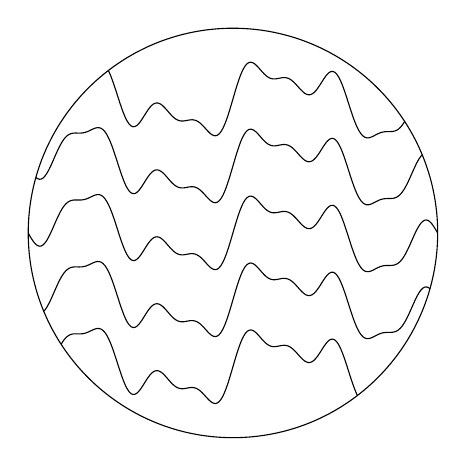
\begin{tikzpicture}[line cap=round]
  % parameters
  \def\R{2.6}   % disk radius
  \def\N{7}     % number of chords
  \def\t{1.0}   % 0 = straight chords, 1 = fully deformed
  \def\A{0.38}  % deformation amplitude (relative to R)

  % spacing of the reference chords
  \pgfmathsetmacro{\step}{2*\R/(\N+1)}

  % a smooth x-only warp (so ordering in y is preserved => no crossings)
  \pgfmathdeclarefunction{warp}{1}{%
    % argument is x/R (dimensionless). trig in radians -> add 'r'
    \pgfmathparse{0.35*sin(2*pi*#1 r) + 0.22*sin(5*pi*#1 r + 0.7) + 0.12*sin(9*pi*#1 r - 0.4)}%
  }

  \begin{scope}
    \clip (0,0) circle (\R);
    \foreach \i in {2,3,4,5,6} {
      \pgfmathsetmacro{\c}{-\R + \i*\step} % reference y-level
      \draw plot [smooth, samples=220, domain=-\R:\R]
        (\x, { \c + \t * \A * \R * warp(\x/\R) + 0.2*(\i-4)});
    }
  \end{scope}

  % boundary last
  \draw (0,0) circle (\R);
\end{tikzpicture}
